\documentclass[a4paper]{exam}

\usepackage{geometry}
\usepackage{graphicx}
\usepackage{hyperref}
\usepackage{mathtools}
\usepackage{titling}

\graphicspath{{images/}}

\printanswers

\title{Weekly Challenge 10: Graph Connectivity\\CS 412 Algorithms: Design and Analysis}
\author{team-name}  % <==== replace with your team name for grading
\date{Habib University | Spring 2023}

\runningheader{CS 412: Algorithms}{WC10: Graph Connectivity}{\theauthor}
\runningheadrule
\runningfootrule
\runningfooter{}{Page \thepage\ of \numpages}{}

\qformat{{\large\bf \thequestion. \thequestiontitle}\hfill}
\boxedpoints

\begin{document}
\maketitle

\begin{questions}

  

\titledquestion{DEI}

  \begin{center}
    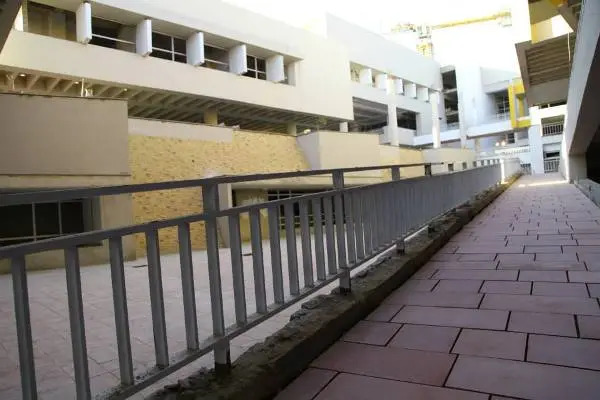
\includegraphics[width=.7\textwidth]{ramp}\\
    \small ``Here Is Why I Chose Habib University'', \href{https://tribune.com.pk/article/22246/here-is-why-i-chose-habib-university}{The Express Tribune}.
  \end{center}

  Following the recent \href{https://www.facebook.com/karachi.usconsulate/posts/pfbid0sb9UC6H9KPnS7fmHSpNQiHQrzXDAFhRKwWRiLD7tjDwQpyuUQKrm6vXfYH2xYUG9l}{speaker on ``Diversity, Equity \& Inclusion''} from the US of A, HU is undertaking an accessibility audit of the city campus and has enlisted a greatest algorithmicist, yourself! You have identified $n$ distinct locations on campus connected by various passages. Each passage is passable with a wheelchair, without a wheelchair, or both. It makes its endpoints mutually reachable.

  In the audit, a passage is \textit{Type A} if it is passable with a wheelchair, and \textit{Type B} if it is passable without a wheelchair. Two locations, $u$ and $v$, are \textit{A-accessible} if there is a sequence of Type A passages between them. A similar definition applies for \textit{B-accessible}.

  The campus is \textit{DEI-compliant} and clears the audit if any two distinct locations, $u$ and $v$, are A-accessible if and only if they are B-accessible.

  \subsection*{Input \& Constraints}
  The first line contains 2 integers, $n$ and $q$. ($1\leq n \leq 10^5, 1\leq q \leq 2\cdot 10^5$)
  \\
  Each of the $q$ subsequent lines specifies a passage of Type A or Type B between $u$ and $v$. ($1\leq u,v \leq n$)
  
  \subsection*{Output}
  Compute and return $q$ \texttt{bool} values. The $i$-th value indicates whether addition of the $i$-th passage makes the campus DEI-compliant.

  \subsection*{Sample}
  \begin{minipage}[t]{.21\textwidth}
    \begin{tabular}[t]{|l|l|}
      \hline
      Input & Output\\
      \hline
      5 8 & \texttt{False}  \\
      A 1 2 & \texttt{False}  \\
      A 2 3 & \texttt{False}  \\
      B 1 3 & \texttt{True}  \\
      B 1 2 & \texttt{False}  \\
      A 3 4 & \texttt{False}  \\
      B 2 5 & \texttt{False}  \\
      A 4 5 & \texttt{True}  \\
      B 1 4 &   \\
      \hline
    \end{tabular}
  \end{minipage}
  \begin{minipage}[t]{.78\textwidth}
    \underline{Explanation}\\
    After the 1st passage is added, locations 1 and 2 are A-accessible but are not B-accessible, so the campus is not DEI-compliant.\\
    The same reasoning applies after adding the 2nd and 3rd passages.\\
    After the 4th passage is added, the campus is DEI-compliant as all pairs of locations are now A-accessible if and only if they are B-accessible.\\
    After the 5th, 6th and 7th passages are added, locations 3 and 4 are A-accessible but not B-accessible.\\
    After the 8th passage is added,  the campus is DEI-compliant as all pairs of locations are now A-accessible if and only if they are B-accessible.\\
  \end{minipage}

  \subsection*{Tasks}
  \begin{enumerate}
  \item Implement the function, \texttt{connect\_campus}, in the accompanying file, \texttt{test\_campus.py}. Pay attention to the parameter and return types.
  \item Run \texttt{pytest test\_campus.py} locally in order to identify and debug any errors.
  \item Adhere to good attribution practices: make sure to cite any sources or references, \href{https://hulms.instructure.com/courses/2616/discussion_topics/29240}{especially if using AI}.
  \end{enumerate}

  \subsection*{Credits}
  This problem is adapted from \href{https://www.hackerearth.com}{HackerEarth}.
  
\end{questions}

\end{document}

%%% Local Variables:
%%% mode: latex
%%% TeX-master: t
%%% End:
